\documentclass{article}
\usepackage{tikz}
\usetikzlibrary{positioning, shapes.geometric, arrows.meta, calc}

\begin{document}

\section{Proposal}

The end goal is to achieve good, aggressive control at the limits from high-dimensional sensor data. Initially, that high-dimensional data will be camera images; in the fullness of time, maybe that also includes LiDAR data, IMU data, etc.

What I'm proposing is model-predictive control (i.e., MPPI) from pixels. During training, when we have access to ground-truth state, we can train an environment model that maps input images to the state variables that we need; a high-level proposal for the design of a deep learning architecture is as follows:

\begin{figure}[h]
\centering
\scalebox{0.7}{
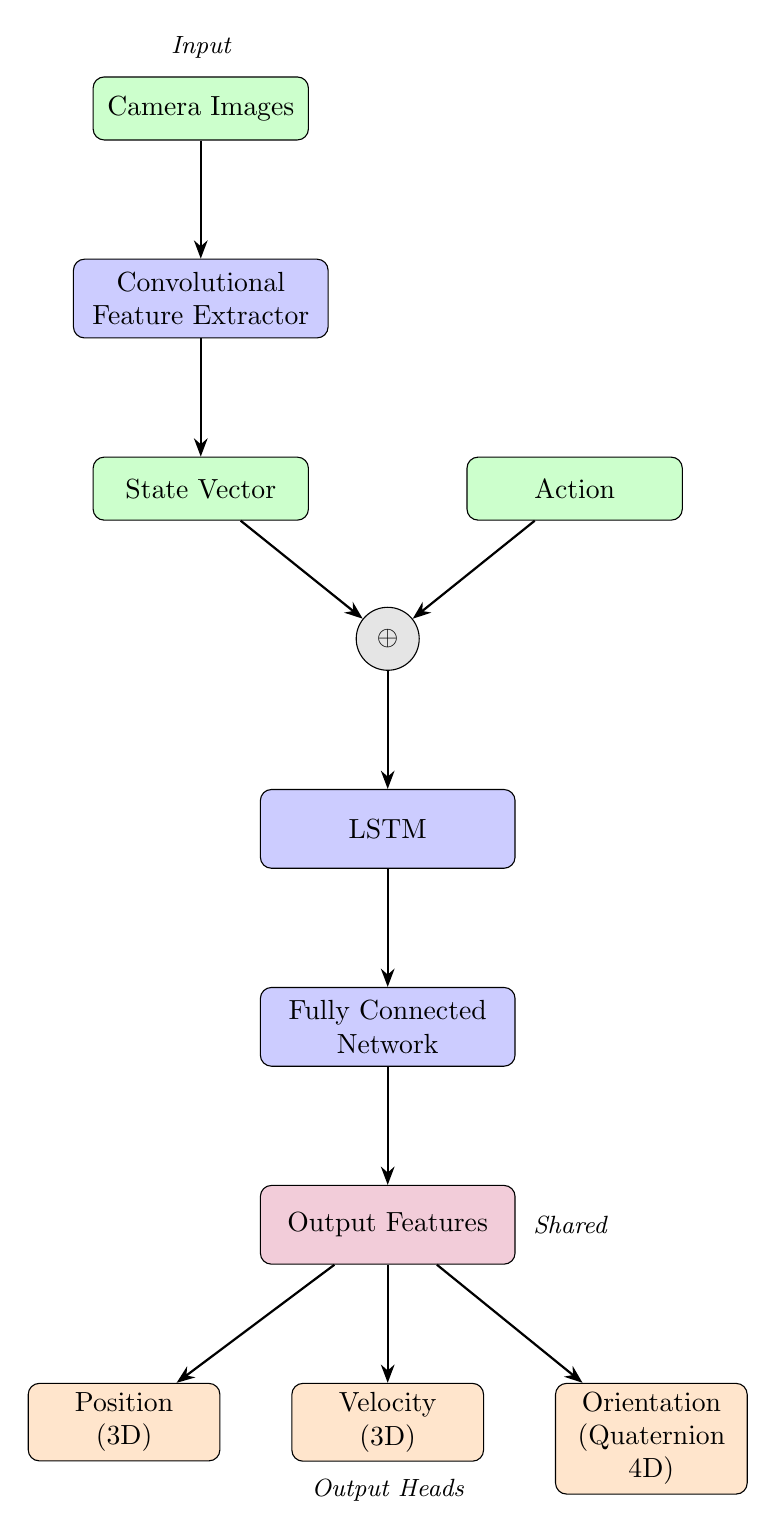
\begin{tikzpicture}[
    node distance=1.5cm,
    block/.style={rectangle, draw, fill=blue!20, text width=3cm, text centered, rounded corners, minimum height=1cm},
    input/.style={rectangle, draw, fill=green!20, text width=2.5cm, text centered, rounded corners, minimum height=0.8cm},
    output/.style={rectangle, draw, fill=orange!20, text width=2.2cm, text centered, rounded corners, minimum height=0.8cm},
    arrow/.style={-Stealth, thick},
    concat/.style={circle, draw, fill=gray!20, minimum size=0.8cm}
]

% Input
\node[input] (camera) {Camera Images};

% Feature Extractor
\node[block, below=of camera] (conv) {Convolutional\\Feature Extractor};

% State vector
\node[input, below=of conv] (state) {State Vector};

% Action input
\node[input, right=2cm of state] (action) {Action};

% Concatenation node
\node[concat, below=1.5cm of $(state)!0.5!(action)$] (concat) {$\oplus$};

% LSTM
\node[block, below=of concat] (lstm) {LSTM};

% FCNN
\node[block, below=of lstm] (fcnn) {Fully Connected\\Network};

% Output features
\node[block, below=of fcnn, fill=purple!20] (features) {Output Features};

% Output heads
\node[output, below left=1.5cm and 0.5cm of features] (pos) {Position\\(3D)};
\node[output, below=1.5cm of features] (vel) {Velocity\\(3D)};
\node[output, below right=1.5cm and 0.5cm of features] (orient) {Orientation\\(Quaternion 4D)};

% Arrows
\draw[arrow] (camera) -- (conv);
\draw[arrow] (conv) -- (state);
\draw[arrow] (state) -- (concat);
\draw[arrow] (action) -- (concat);
\draw[arrow] (concat) -- (lstm);
\draw[arrow] (lstm) -- (fcnn);
\draw[arrow] (fcnn) -- (features);
\draw[arrow] (features) -- (pos);
\draw[arrow] (features) -- (vel);
\draw[arrow] (features) -- (orient);

% Labels
\node[above=0.1cm of camera, font=\small\itshape] {Input};
\node[right=0.1cm of features, font=\small\itshape] {Shared};
\node[below=0.1cm of vel, font=\small\itshape] {Output Heads};
\end{tikzpicture}
}
\caption{Proposed deep learning architecture}
\end{figure}

This is a high-level diagram, and the details will probably need to be fleshed out as results come in. The output is the state vector necessary for model-predictive control, with which we can run the model-predictive controller.

\end{document}
